 \documentclass[paper=a4, pagesize, DIV=calc, BCOR=12.5mm, twoside=on, onecolumn=on, open = any, titlepage =on, parskip =half-, headsepline = on, footsepline = on, chapterprefix = on, appendixprefix = off, fontsize = 12pt, numbers = noenddot, abstract = on]{scrbook}
\usepackage[utf8]{inputenc}
\usepackage[german]{babel}
\usepackage{amsmath}
\usepackage{amsthm}
\usepackage{amsfonts}
\usepackage{amssymb}
\usepackage{makeidx}
\usepackage{graphicx}
\usepackage{tikz}
\usepackage{wrapfig}
\usepackage{geometry}
\usepackage{parallel}
\usepackage{todonotes}
 \usepackage{mathptmx}
 \usepackage{pdfsync}
 \usepackage{url}
 \usepackage{float}
 \usepackage{hyperref}

 %\usepackage[scaled=.90]{helvet}
 \usepackage[T1]{fontenc} 
%\newcommand{\changefont}[3]{ \fontfamily{#1} \fontseries{#2} \fontshape{#3} \selectfont}
%\changefont{cmr}{m}{n} %ppl for Palatino, ptm for Times New Roman
\setkomafont{title}{\rmfamily \bfseries}
\setkomafont{chapterentry}{\rmfamily \bfseries}
\usepackage{cutwin}
\usepackage[raggedleft]{titlesec}
\titlelabel{\thetitle.\quad}
\titleformat*{\chapter}{\scshape\bfseries\large}
\titleformat*{\section}{\bfseries\large}
\titleformat*{\subsection}{\bfseries \normalsize}
\titleformat*{\subsubsection}{\bfseries \normalsize}

\DeclareMathOperator{\GL}{GL} % einige Macro, siehe am Ende Abschn. 2
\newcommand{\N}{\mathbb{N}}
\newcommand{\Z}{\mathbb{Z}}
\newcommand{\Q}{\mathbb{Q}}
\newcommand{\R}{\mathbb{R}}
\newcommand{\C}{\mathbb{C}}
\newcommand{\cP}{{\mathcal P}} 






\numberwithin{equation}{chapter}
%\usepackage{fancyhdr}
%\pagestyle{fancy}
%\fancyhead{}
%\fancyhead[RO,LE]{\thepage}
%\fancyhead[RE]{\thechapter }
%\fancyhead[LO]{\thesection }
%\fancyfoot{}
%\fancyfoot[LE,RO]{Pamina M. Berg}  %Hier muss noch etwas geändert werden...
\usepackage{blindtext}
\usepackage{todonotes}

%\usepackage[german]{babel}
\usepackage[german]{babel}
\usepackage{setspace}
\theoremstyle{definition}
\newtheorem{definition}{Definition}
\theoremstyle{plain}
\newtheorem{beispiel}{Example}
\theoremstyle{plain}
\newtheorem{satz}{Theorem}
\theoremstyle{remark}
\newtheorem{bemerkung}{Remark}
\theoremstyle{plain}
\newtheorem{cor}{Corollary}
\theoremstyle{plain}
\newtheorem{prop}{Proposition}

\begin{document}
\newpage
\thispagestyle{plain}

\pagenumbering{Roman}
\newcommand*\diff{\mathop{}\!\mathrm{d}}

\begin{titlepage}


\begin{figure}[htbp]
		\begin{minipage}[b]{25mm}
			
\includegraphics[width=25mm,clip]{images/logo_uhh}
		\end{minipage}
		\begin{minipage}[b]{2mm}
			
\includegraphics[width=1mm,height=25mm]{images/greypixel}
		\end{minipage}
		\begin{minipage}[b]{12.5cm}
			{   
				\vspace{2mm}
				{\Large Universität Hamburg } \\
				Fakultät für Mathematik,\\
				Informatik und Naturwissenschaften \\
				Department Informatik \\
			}
		\end{minipage}
	\end{figure}


\begin{center} 
\vspace{0.5cm} 
\begin{tabular}{c}
% \vspace{0.5cm}\\
\Large \textsc{Entwicklung einer Java Simulationsumgebung}\\
 \\
\Large \textsc{für Lego Mindstorms NXT Roboter}\\
\\
\\
\small Masterarbeit im Fach Informatik zur Erlangung des akademischen Grades\\
\\
\normalsize \textbf{Master of Education}\\
\\
\small im Studiengang Lehramt an Gymnasien M.Ed.\\
\\
\\
\large \textbf{Pamina Maria Berg}\\
\small \emph{Matr.Nr. 6087438}\\
\\
\normalsize Hamburg, den \today
\end{tabular}
\par 
\end{center}
\par
\vspace*{3cm}
\begin{tabular}{l}
\emph{Erstgutachter}\\
Dr.\, Guido Gryczan\\
\emph{Zweitgutachter}\\
Jun.-Prof.\, Dr. Maria Knobelsdorf\\
\emph{Betreuer}\\
Till Aust\\
Fredrik Winkler\\
\end{tabular}

\end{titlepage}


\thispagestyle{empty}
\cleardoublepage



\newpage
\listoffigures
\newpage
\tableofcontents
\thispagestyle{empty}
\cleardoublepage
\newpage
\pagenumbering{arabic}
\par \singlespacing
\chapter{Einleitung}
\onehalfspacing
Die Arbeit mit Robotern bereichert den Informatikunterricht und das Nachmittagsprogramm vieler Schulen seit Jahren. Auf spielerische Art und Weise sollen Schülerinnen und Schüler (im Folgenden SuS abgekürzt) mit einfachen Konstrukten der objektorientierten Programmierung umzugehen lernen. Dies geschieht zum einen mit Drag-and-Drop Softwareangeboten wie das standardmäßig mit ausgelieferte NXT Mindstorms Tool \todo{Referenz:NXT Software}, oder auch Enchanting. \todo{Referenz: Enchanting} Zum anderen bietet sich ab der Mittelstufe (Klasse 7 -- 10) die Arbeit mit BlueJ zur Erstellung erster selbstgeschriebener Programme an. Hierzu kann eine BlueJ Extension genutzt werden, die mit der Java Virtual Machine leJOS NXJ für NXT Roboter arbeitet.\\

Doch immer wieder stoßen Lehrkräfte in den Schulen auf Hardwareprobleme jeglicher Art, wie zum Beispiel das Fehlen von einer ausreichenden Anzahl an Robotern im Unterricht oder auch fehlende Firmwareupdates oder defekte Sensoren.\\
Auch ist das Zusammen- und wieder Auseinanderbauen der Roboter ein Aufwand, der nicht für den alltäglichen Unterricht geeignet ist. Um kleine Aufgaben mit Java zu lösen, wie zum Beispiel das Fahren einer S-Kurve oder das Anhalten auf einem bestimmten Punkt, muss bisher immer erst der Roboter gestartet, der Code in BlueJ verfasst, auf den Roboter übertragen und dieser dann zu einem geeigenete Parcours gebracht werden.\\

Um diese Probleme zu umgehen und den Einstieg in die objektorientierte Programmierung über die Benutzung von LEGO Mindstorms Robotern zu ermöglichen, soll im Rahmen dieser Masterarbeit eine Simulationsumgebung für die Arbeit mit LEGO Mindstorms NXT Roboter entstehen.\todo{Referenz}
\newpage
\par\singlespacing
\chapter{Ausgangssituation}

\par\singlespacing
\section{Das LEGO Mindstorms NXT System}
\onehalfspacing
Die ersten computergesteuerten LEGO Produkte wurden bereits 1986 veröffentlicht. In einer Zusammenarbeit von LEGO Education und dem Massachussettes Institute of Technology (MIT) wurde LEGO TC LOGO entwickelt. Dies war eine spezielle Abwandlung der Programmiersprache LOGO, mit der zusammengesetzte LEGO-Modelle gesteuert werden konnten \cite{rolling:14}.\\
Die Entwicklung eines programmierbaren LEGO-Steins begann 1988 und erreichte ihren Höhepunkt mit der Vorstellung des ersten MINDSTORMS Systems im Januar 1998, bei der der LEGO MINDSTORMS RCX Intelligent Brick, ein Microcomputer und somit das Kernstück des RCX-Systems, und das Robotics Invention System im Museum of Modern Art in London vorgestellt wurden.\\
Bereits zwei Monate nach Verkaufsstart wurde die FIRST LEGO League (FLL) gegründet -- eine Zusammenarbeit zwischen LEGO und FIRST (For Inspiration and Recognition of Science and Technology), die den Grundstein für die heute noch bestehende Wettbewerbsliga legte \cite{rolling:14}.\\
Die Vorstellung und der Verkaufsstart der Nachfolge-Roboter des RCX-Systems, den LEGO MINDSTORMS NXT Robotern, fand im August 2006 statt. Diese damals neu entwickelten Roboter sind auch, dank eines Updates in 2009, fast zehn Jahre später noch in den Schulen und Universitäten zu finden. Im April 2005 fand die erste FLL Weltmeisterschaft in Atlanta, Georgia, statt und bis heute bieten die Weltmeisterschaften einen Anlaufpunkt für Jugendliche auf der ganzen Welt, die ihr Können und ihre Roboter auf die Probe stellen wollen \cite{lego}.

\par \singlespacing
\section{Die Arbeit mit LEGO-Robotern im Unterricht}
\onehalfspacing
Die Robotik als Teilgebiet der Informatik in der Schule gewinnt zunehmend an Bedeutung. Nicht nur die Programmierung steht im Vordergrund, sondern auch die Kompetenz, Probleme unter bestimmten Aufgabenstellungen zu lösen. \textsc{Berns} und \textsc{Schmidt}, die Verfasser eines der Kernwerke für den Unterricht mit dem LEGO MINDSTORMS System, schreiben, dass bei der Arbeit mit Robotern im Unterricht "`durch eine konkrete Aufgabenstellung, das problemspezifische Konstruieren und Programmieren eines Roboters sowie durch das letztendliche Testen der gesamte Ablauf eines Problemlösungsprozesses kennen gelernt"' \cite[S.2]{berns:10} wird.\todo{An dieser Stelle kann noch auf die Kooperation \cite{wagner:05} eingegangen werden}\\

Es erfolgt nun zunächst die curriculare Einordnung des Themas Roboter im Unterricht in die Bildungspläne aus Hamburg. Danach werden verschiedene Arbeitsmethoden im Zusammenhang mit dieser Art von Unterricht vorgestellt.

\subsection{Curriculare Einordnung}
Die fachlichen Inhalte, die mithilfe des Einsatzes von Robotern im Unterricht vermittelt werden können, sind sowohl im Bildungsplan der Sekundarstufe I für das Gymnasium (Klasse 7 -- 10) und die Stadtteilschule (Klasse 7 -- 11), als auch im Bildungs- bzw. Rahmenplan für die Gymnasiale Oberstufe, der Sekundarstufe II, verankert.

\subsubsection{Gymnasium Sekundarstufe I (7 -- 10) Informatik Wahlpflicht}
Der Einsatz von Robotern kann auf die Module 2 und 3 des Bildungsplanes für die Sekundarstufe I des Gymnasiums bezogen werden. Hier heißt es\\

\emph{Modul 2}
\begin{itemize}
\item \emph{Abläufe analysieren und umgangssprachlich beschreiben, zu Algorithmen formalisieren und mit einer formalen Sprache implementieren}
\item \emph{Umgang mit einer einfachen Entwicklungsumgebung}
\item \emph{Testen, Ergebnisse interpretieren und bewerten}
\item \emph{Grundlagen der prozeduralen Programmierung: Sequenz, Alternative, Wiederholung, Prozedur bzw. Funktion}
\end{itemize}

\emph{Modul 3 -- Kontext Daten und Prozesse}
\begin{itemize}
\item \emph{Grundlagen der prozeduralen Programmierung}
\item \emph{Abläufe formalisieren}
\item \emph{Algorithmen mit einer formalen Sprache implementieren}
\item \emph{Testen, Ergebnisse interpretieren und bewerten}
\end{itemize}

\todo{Zitat Bildungsplan}

\subsubsection{STS Sekundarstufe I (7 --11) Informatik}
Ähnlich ist es im Bildungsplan für die Stadtteilschulen. Hierbei werden allerdings innerhalb der Module verbindliche Inhalte formuliert.\\
So sind im Modul 2 die Inhalte \emph{Algorithmen} und \emph{prozedurale Programmierung: Sequenz, Alternative, Wiederholung, Funktion} zu finden, die, wie der Bildungsplan vorschlägt, in das Unterrichtsvorhaben \emph{"Wir lassen Roboter arbeiten"} integriert werden können.\\
Im Modul 3 sollen im zweiten Halbjahr die verbindlichen Inhalte
\begin{itemize}
\item \emph{Grundlagen der prozeduralen Programmierung}
\item \emph{Abläufe formalisieren}
\item \emph{Algorithmen mit einer formalen Sprache implementieren}
\item \emph{Testen, Ergebnisse interpretieren und bewerten}
\end{itemize}
unterrichtet werden. 
\todo{Quelle}

\subsubsection{Gymnasiale Oberstufe -- Vorstufe}

In der Vorstufe sollen sich die SuS mit den Inhalten des Moduls \emph{Daten und Prozesse} beschäftigen. Diese beinhalten das Analysieren und umgangssprachliche Bescheiben von Abläufen, das Strukturieren von Daten sowie die Verwendung von Variablen und Parametern, das Formalisieren von Abläufen, die Grundlagen der prozeduralen Programmierung, die Implementation von Algorithmen mit einer formalen Sprache, das Testen und das Interpretieren und Bewerten von Ergebnissen. \todo{Quelle}

\subsubsection{Gymnasiale Oberstufe -- Studienstufe}

In der Studienstufe gibt es den verbindlichen Inhalt \emph{Objektorientierte Modellierung}, der die folgenden Punkte umfasst:\\
\begin{itemize}
\item \emph{Idee des OO-Konzepts mit Objekten und ihrer Kommunikation, Vererbung und Nutzerbeziehung}
\item \emph{Erarbeitung der Sprachelemente der verwendeten objektorientierten Programmiersprache, Berücksichtigung von Programmierkonventionen, Nutzen von Bausteinen/Libraries}
\item \emph{Nutzung einer IDE mit UML-Diagrammen und Quellcode zur schrittweisen Implementierung eines Informatiksystems.}
\end{itemize}
\todo{Zitat}

\subsubsection{Genereller Einsatz von Robotern als Hilfsmittel im Unterricht}
Da laut Bildungsplan die projektorientierte Arbeit in Informatik in der Studienstufe einen bedeutenden Stellenwert hat, bietet es sich natürlich an, eine Projektarbeit zum Thema \emph{Einsatz von Robotern} mit Bezug auf verschiedene Ligen (schulisch und universitär) zu gestalten, bei der als Produkt eine bestimmte Aufgabe mit den Robotern erledigt werden soll. \todo{Quelle?}\\

Die einfachste Methode, um SuS an die problemorientierte Arbeitsweise im Rahmen der Programmierung mit Robotern heranzuführen ist der Einsatz von so genannten \emph{Use Cases}. Hierbei handelt es sich um aus der Realwelt gegriffene \todo{anderes Wort} Situationen, die in unserem Fall mithilfe des Roboters bewältigt werden sollen. Ein klassischer Use Case für den Einstieg wäre die Situation, dass der Roboter vor einem Hindernis steht, um das er herumfahren soll. Hierbei kann man den SuS vorgeben, dass sie z.B. im Viereck um das Hindernis herum navigieren sollen.
Ein weitaus komplexerer Use Case bietet sich im Zusammenhang mit der RoboCup Wettbewerbsliga \emph{Rescue} an, in der ein in einem Labyrinth verstecktes Opfer gerettet werden soll. Hierbei würden sich nun die SuS damit beschäftigen, wie sie durch das Labyrinth navigieren, wie sie Hindernissen ausweichen, und welche bautechnischen Spezifikationen ihr Roboter haben muss, um das Opfer an einen sicheren Ort zu transportieren.

\section{Bisher verfügbare Softwarelösungen}
\label{sec:software bisher}
In diesem Kapitel wird nun eine Auswahl von verfügbaren und im Unterricht getesteten Softwarelösungen zur Programmierung der NXT Roboter vorgestellt.

\subsection{LEGO Mindstorms NXT}
\label{sec:LMNXT}

Das LEGO Mindstorms NXT-Programm ist eine von der Firma LEGO zur Verfügung gestellte Programmieroberfläche für NXT-Roboter. 

\begin{figure}[htbp]
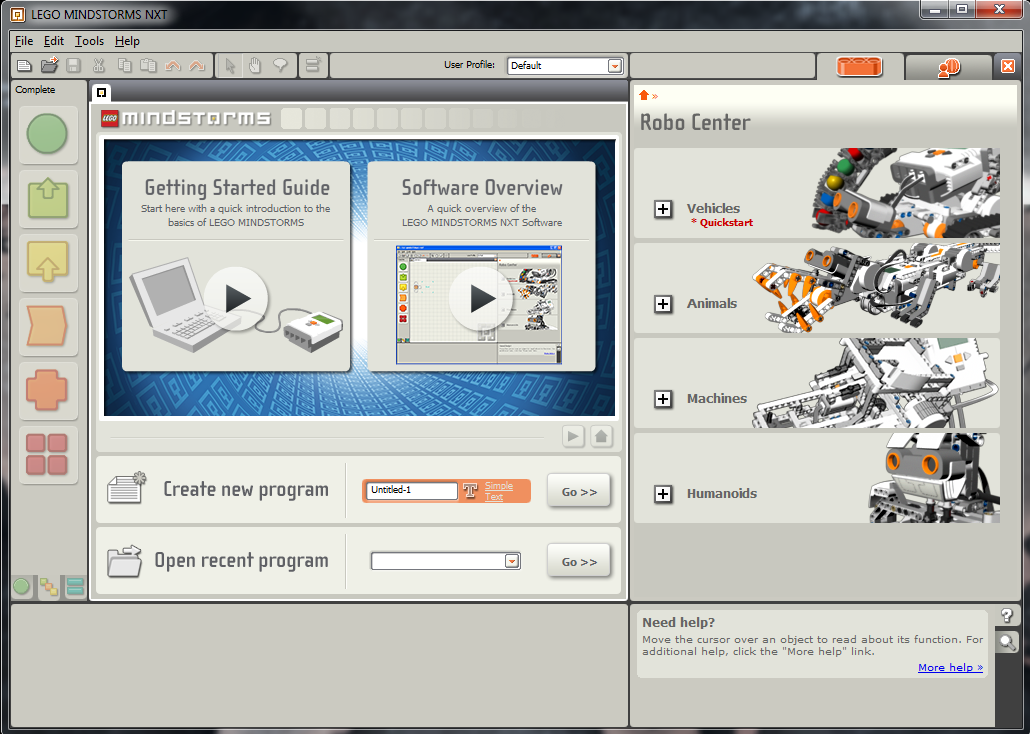
\includegraphics[scale=0.54]{images/Startbildschirm_NXT.png} 
\caption{Der Startbildschirm des LEGO Mindstorms NXT-Programms}
\label{fig:NXT Start}
\end{figure}

Die Abbildung \ref{fig:NXT Start} zeigt den Startbildschirm der Entwicklungsumgebung. Dieser stellt neben zwei Videoanleitungen als Hilfe für Anfänger auch das \emph{Robo Center} zur Verfügung, in dem verschiedene von LEGO vorgeschlagene Roboter-Modelle, die mithilfe des Bausatzes des NXT zusammengesetzt werden können, vorgestellt werden \todo{Was passiert hier noch?}.\\
Sobald eine neue oder bestehende Programmdatei geöffnet wird, können die SuS mithilfe von Blöcken, die unter anderem der Bewegung und Sensorik dienen und dabei einfache Steuerungsmechanismen sowie Elemente der Regelungstechnik zur Verfügung stellen, ihren Roboter programmieren.

\begin{figure}[htbp]
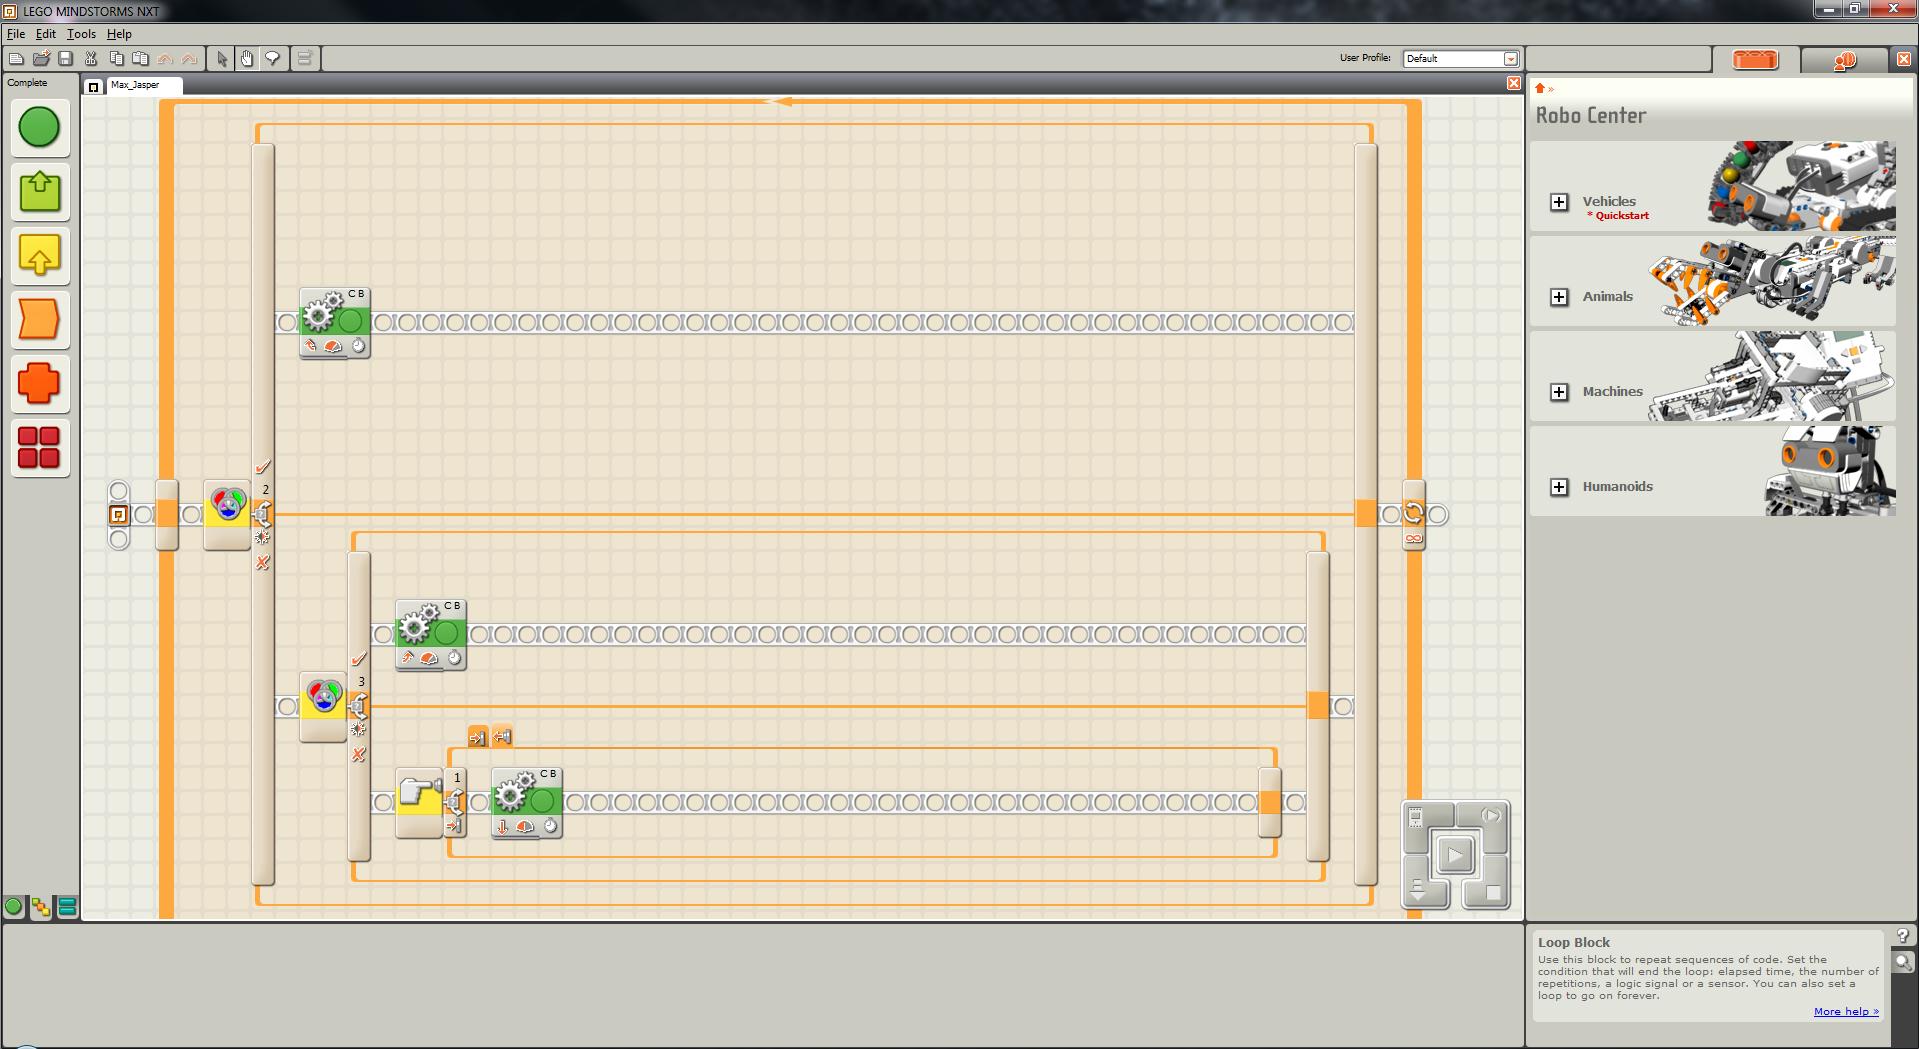
\includegraphics[scale=0.281]{images/Beispielprogramm_NXT.png} 
\caption{Fahren eines Roboters auf einer schwarzen Linie}
\label{fig:Bsp NXT}
\end{figure}

\subsection{Enchanting}
\label{sec:enchanting}

Enchanting ist eine an \emph{Scratch} anknüpfende Entwicklungsumgebung. Wie das in \textbf{\ref{sec:LMNXT}} beschriebene Programm wird auch hier mithilfe von Drag-and-Drop gearbeitet. 

\begin{figure}
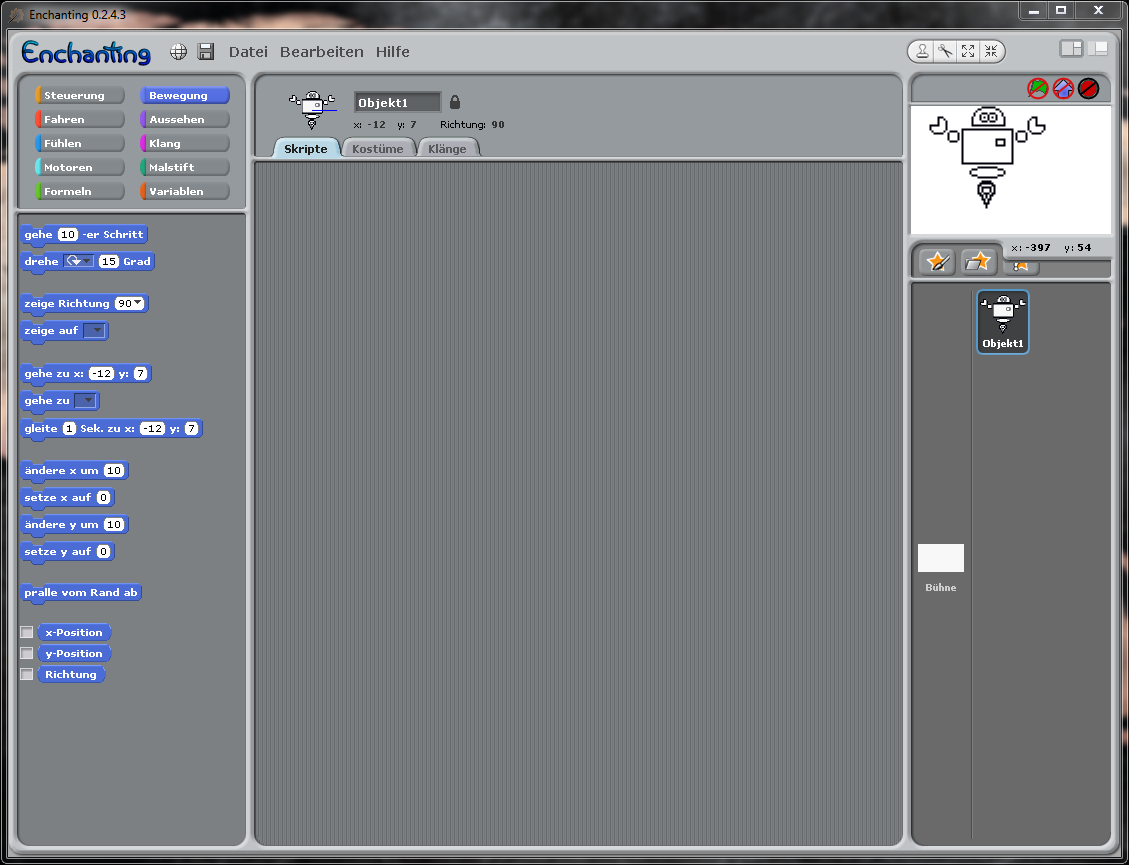
\includegraphics[scale=0.5]{images/Enchanting_Start.png} 
\caption{Der Startbildschirm von Enchanting}
\label{fig:Enchanting Start}
\end{figure}

\begin{figure}
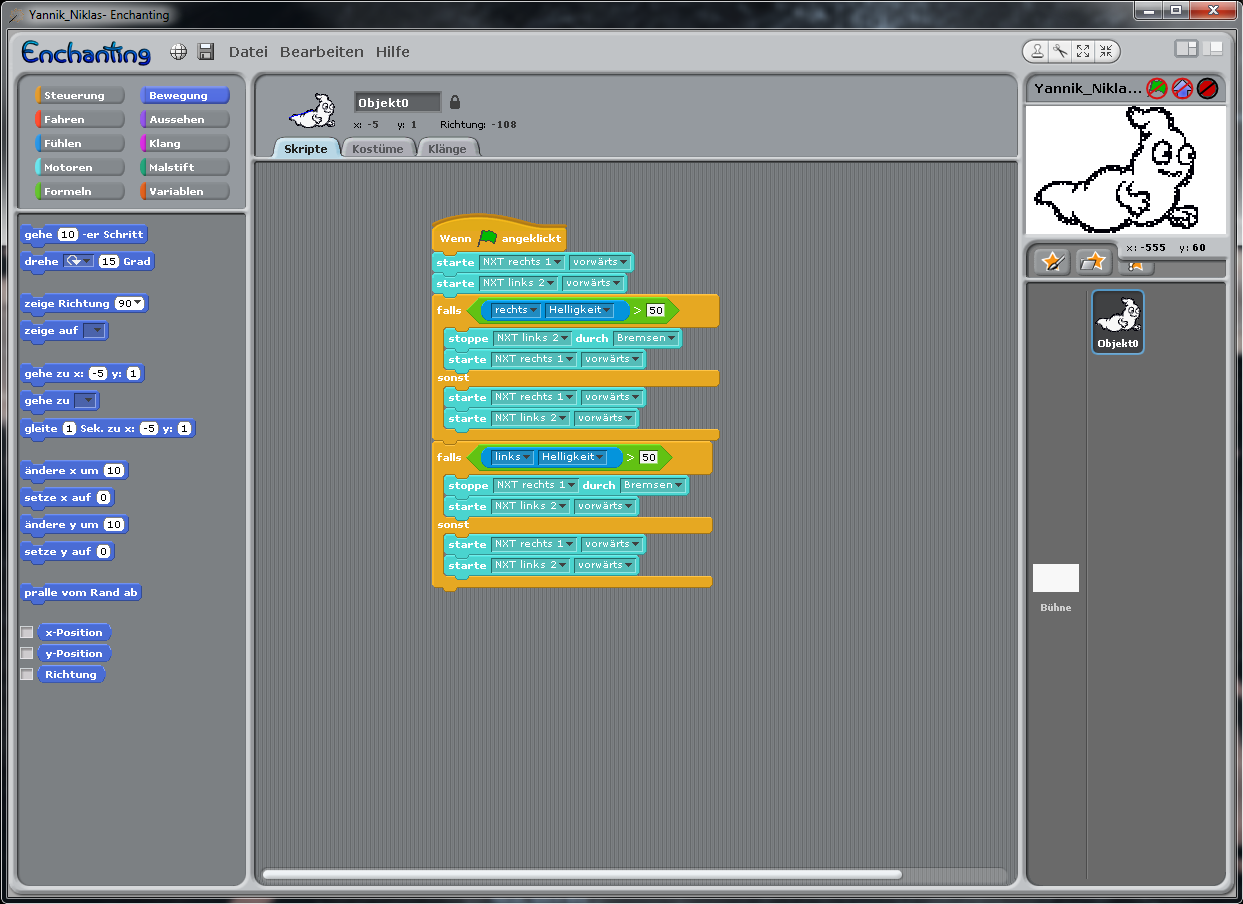
\includegraphics[scale=0.45]{images/Beispielprogramm_Enchanting.png} 
\caption{Beispiel eines Enchanting Programms}
\label{fig:Bsp Enchanting}
\end{figure}


\subsection{BlueJ}
\label{sec:bluej}

\par \singlespacing
\section{leJOS}
\label{sec:lejos}
\onehalfspacing
leJOS ist eine kleine Java Virtual Machine und stellt alle Klassen der NXJ API zu Verfügung, mithilfe derer Lego Mindstorms NXT Roboter in Java programmiert werden können \cite{lejos}.


\par \singlespacing
\chapter{Anforderungen an die Neuimplementierung}
\label{chap:anforderungen}
\onehalfspacing
Nicht nur in der Schule, sondern insbesondere in der Wissenschaft spielt Simulation in der Robotik eine wichtige Rolle \cite[S.13]{hertzberg:12}. Die Anforderungen, die an die wissenschaftlichen Simulationsumgebungen der Robotik gestellt werden, fassen \textsc{Hertzberg, Lingemann} und \textsc{Nüchter} wie folgt zusammen:
\begin{itemize}
\item \emph{"`Die Umgebung muss hinreichend gut simuliert sein. Die Simulation einer Flughafenterminalhalle muss zum Beispiel "`zufällig"' umherlaufende Fluggäste mit Gepäck und Transportkarren umfassen.}
\item \emph{Der Roboter in seiner Funktionalität muss hinreichend gut simuliert sein. Das betrifft seine Aktionen wie auch seine Sensorik.}
\item\emph{Relevante Ungenauigkeit technischer Sensoren und Effektoren muss abgebildet werden. Kann zum Beispiel im realen Bild einer Kamera auf dem Roboter ein Orientierungspunkt im Gegenlicht der Fensterfront unsichtbar werden, muss die Simulation diesen Effekt reproduzieren.}
\item \emph{Die "`Wahrheit"' im Simulator ist tabu! Natürlich ist im Simulator der Zustand jedes simulierten Objekts präzise bekannt, einschließlich der Position, Richtung und Geschwindigkeit des Roboters. Die Roboterkontrollsoftware darf hierauf nicht zugreifen, um Information über die Umgebung zu erhalten -- das geht nur über die simulierten Sensoren. (Für die externe Bewertung des Roboterverhaltens ist der Vergleich zwischen der Wahrheit im Simulator und der Information in der Roboterkontrollsoftware aber erlaubt.)}
\item \emph{Der Simulator sollte für den simulierten Roboter die identische Schnittstelle wie der reale Roboter zwischen Roboterkontrollsoftware einerseits und Robotersensorik und -aktuatorik andererseits verwenden; die Roboterkontrollsoftware soll also code-identisch für den realen oder den simulierten Roboter verwendet werden."'} \cite[S.14]{hertzberg:12}
\end{itemize}

In den folgenden beiden Unterkapiteln werden nun die Anforderungen an die Neuimplementierung des Simulator-Prototyps für LEGO Mindstorms NXT Roboter aus Sicht der Schüler und und der Lehrer dargestellt, sowie Parallelen und Unterschiede zu den oben dargestellten herausgearbeitet.

\section{Schülerperspektive}
\label{sec:schüler}
\onehalfspacing
Da es sich bei der Simulationsumgebung um einen Prototypen handelt, der möglicherweise schon ab der fünften, regelmäßig aber ab der siebten Klasse eingesetzt werden soll, steht ein Augenmerk ganz besonders im Fokus: die Einfachheit. Sowohl in der Bedienung des Simulators als auch im Aussehen sollten klare und leicht erkennbare Strukturen vorherrschen.\\
Des weiteren sollte darauf geachtet werden, dass die SuS für die Programmierung des Roboters und die Benutzung des Simulators eine einheitliche Syntax verwenden können. Hierzu muss die Simulationsumgebung genau die Methoden anbieten, die auch bei dem realen Roboter die Steuerung der Motoren und den Zugriff auf Sensordaten ermöglichen. Dies entspricht dem zweiten Aspekt nach \textsc{Hertzberg et al.}, da der simulierte Roboter alle für die Arbeit mit SuS zentralen Funktionen anbieten und sich hinreichend ähnlich wie ein Roboter in der Realwelt verhalten soll. Des weiteren wird hiermit auch der Aspekt der code-identischen Roboterkontrollsoftware erfüllt, da die SuS das selbe Programm für den Simulator, wie auch für den Roboter selbst benutzen können sollten.\\
Ein weiterer Aspekt, den \textsc{Hertzberg et al.} beschreiben sind die Parcours selbst. Diese sollten möglichst realitätsgetreu umgesetzt werden. Das heißt, dass Ausschnitte eines bestehenden realen Wettbewerbsparcours genutzt werden könnten, um für die SuS eine möglichst realitätsnahe Testumgebung anzubieten.\\
\par \singlespacing
\section{Lehrkraft}
\label{sec:lehrkraft}
\par \onehalfspacing
Für Lehrkräfte ist es erfahrungsgemäß wichtig, dass die Simulationsumgebung alle essentiellen Bausteine der objektorientierten Programmierung im Kontext der Lego-Roboter zur Verfügung stellt. Hierzu gehört das Austesten des Fahrens mithilfe einer Schleife, sowie der verschiedenen Sensoren. Hierzu sollte es eine Auswahl an verschiedenen Parcours geben, damit der Fokus bei jedem Parcours auf einer einzigen Sache liegt. Sollen etwa die angebauten Lichtsensoren getestet werden, so bietet es sich an, den Parcours einfach aus einem weißen Hintergrund und einer schwarzen Linie, die entweder senkrecht in der Nähe des Roboters platziert ist, oder als S-Kurve eine Teilstrecke des realen Labyrinths darstellt, bestehen zu lassen.\\
Des weiteren ist es wichtig, dass sich Lehrerinnen und Lehrer schnell in die Simulationsumgebung einarbeiten können, um bei Fragen der SuS sofort Hilfe leisten zu können.

\par \singlespacing
\section{Erweiterbarkeit} \label{sec:erweiterbarkeit}
\onehalfspacing




\chapter{Entwickelte Software}



\section{Beschreibung der Software}

\subsection{Lichtsensoren}
Die Lichtsensoren sind zwei von der leJOS-API vorgegebene Exemplare der Klasse LightSensor. Diese sind im Prototyp der Simulation jeweils im Abstand von fünf Pixeln links und rechts von der Spitze des Roboter-Dreiecks angebracht. Da es sich bei der Implementation um einen Prototyp handelt, gibt es noch keine optische Repräsentation der beiden Sensoren am Roboter.\\
Die Klasse \texttt{Roboter} enthält die Methoden zur Abfrage der Positionen der Sensoren im Bezug auf die x- und y-Achse: \texttt{gibXLichtRechts()}, \texttt{gibYLichtRechts()},\\
\texttt{gibXLichtLinks()} und \texttt{gibYLichtsLinks()}. Diese werden benötigt, um das Auslesen des Farbwerts des Pixels unter dem jeweiligen Sensor zu ermöglichen.

\section{Softwarearchitektur}

\newpage
\chapter{Zusammenfassung und Ausblick}

\newpage
\begin{thebibliography}{ABCD}

\renewcommand{\refname}{\normalsize Literaturverzeichnis}

\bibitem[Abe01]{abend:01}
Michael Abend. "'Robotik und Sensorik. Darstellungsschwerpunkt: Selbständige Entwicklung "`unscharfer"' Algorithmen zur räumlichen Orientierung (unter Verwendung des LEGO-Mindstorms-Systems)", \emph{Schriftliche Prüfungsarbeit zur zweiten Staatsprüfung für das Amt des Studienrats}, Berlin, 2001

\bibitem[Her12]{hertzberg:12}
Joachim Hertzberg, Kai Lingemann, Andreas Nüchter. \emph{Mobile Roboter. Eine Einführung aus Sicht der Informatik}, Springer-Verlag Berlin Heidelberg, 2012

\bibitem[Hub07]{hubwieser:07}
Peter Hubwieser. \emph{Didaktik der Informatik}, 3. Auflage, Springer-Verlag Berlin Heidelberg, 2007

\bibitem[Lego]{lego}
o.V. URL: \url{http://www.lego.com/en-us/mindstorms/history}, Abgerufen am 06.11.2015, LEGO, 2015

\bibitem[leJOS]{lejos}
o.V. URL: \url{http://www.lejos.org/nxj.php}, Abgerufen am 14.12.2015, leJOS Java for Lego Mindstorms, 2015

\bibitem[Nie99]{nievergelt:99}
Jürg Nievergelt. \emph{"Roboter programmieren" - ein Kinderspiel. Bewegt sich auch etwas in der Allgemeinbildung?}, Informatik-Spektrum 22:5, S. 364--375, 1999

\bibitem[Rol14]{rolling:14}
Mark Rollins. \emph{Beginning LEGO MINDSTORMS EV3}, Apress, Berkeley, CA, 2014

\bibitem[Sch04]{schreiber:04}
Rafael Schreiber. "Der Einsatz von LEGO-Mindstorms im Informatikunterricht der 11. Klasse der Leonard-Bernstein-Oberschule. Sicherung und Transfer grundlegender algorithmischer Strukturen in NQC.", \emph{Schriftliche Prüfungsarbeit im Rahmen der zweiten Staatsprüfung für das Amt des Studienrats}, Berlin, 2004

\bibitem[Sto01]{stolt:01}
Matthias Stolt. "Roboter im Informatikunterricht", 2001

\bibitem[Wag05]{wagner:05}
Oliver Wagner. "LEGO Roboter im Informatikunterricht. Eine Untersuchung zum Einsatz des LEGO-Mindstorms-Systems zur Steigerung des Kooperationsvermögens im Informatikunterricht eines Grundkurses (12. Jahrgang, 2. Lernjahr) der Otto-Nagel-Oberschule (Gymnasium)", \emph{Schriftliche Prüfungsarbeit im Rahmen der zweiten Staatsprüfung für das Amt des Studienrats}, Berlin, 2005

\end{thebibliography}
\newpage
\thispagestyle{empty}
\vspace*{\fill}
"Hiermit versichere ich, dass ich die Arbeit selbstständig verfasst und keine anderen als die angegebenen Hilfsmittel – insbesondere keine im Quellenverzeichnis nicht benannten Internet-Quellen – benutzt habe, die Arbeit vorher nicht in einem anderen Prüfungsverfahren eingereicht habe und die eingereichte schriftliche Fassung der auf dem elektronischen Speichermedium entspricht."\\

Hamburg, \today \hspace*{\fill} \dots \dots \dots \dots \dots \dots \dots\\
\hspace*{\fill} Pamina Maria Berg $\,$
\end{document}